\documentclass[12pt]{article}
\bibliographystyle{plainnat}
\usepackage[margin=1in]{geometry}
\usepackage[utf8]{inputenc}
\usepackage{graphicx}
\usepackage{setspace}
\usepackage{geometry}
\usepackage[colorlinks=true, linkcolor=blue, citecolor=blue, urlcolor=blue]{hyperref}
\usepackage[square, numbers]{natbib}
\usepackage{multicol}
\usepackage{changepage}  
\usepackage{tabularx}
\usepackage{booktabs}
\usepackage{multirow}
\usepackage{amsmath} 
\usepackage{url} 
\usepackage{hyperref} 
\usepackage{float}
\usepackage{lipsum}
\usepackage{tablefootnote}
\usepackage{xcolor}
\usepackage{array} 
\usepackage{dutchcal}
\usepackage{subcaption} 
\usepackage{natbib} 
\usepackage{soul} 
\usepackage{xcolor} 
\usepackage{titlesec}
\geometry{left=0.7in,right=0.7in,top=0.7in,bottom=0.7in}
\setlength{\parindent}{20pt}
\setlength{\parskip}{0.2em}
\titlespacing*{\section}
  {0pt}         % Left indentation
  {0.2\baselineskip}  % Space before 
  {0.2\baselineskip}  % Space after 
\titlespacing*{\subsection}
  {0pt}
  {0.1\baselineskip}
  {0.1\baselineskip}


\begin{document}
\onehalfspacing
\begin{titlepage} \noindent
    Blind Candidate Number: \par
        \begin{centering}
    {\vspace*{6cm}\huge \textbf{Infrastructure effects by gender in developing countries}
    }\par
    \vspace{3cm}
    \noindent
    \textbf{\large{Abstract}} \par
    \noindent Electricity outages are prevalent in Sub-Saharan Africa. They disrupt daily life, raise firm costs, and lower productivity and employment. To promote and inform investments in electricity reliability, this dissertation estimates the effect of outages on equilibrium employment and identifies vulnerable groups. On the labour supply side, I find support for a hypothesis implying women’s employment is more vulnerable. I then use an instrumental variable strategy to estimate the net effect, finding that outages decrease employment more for men than women. To reconcile these, I consider demand, arguing that energy-intensive manufacturing occupation is partly responsible for male workers' vulnerability to outages. \end{centering}
        \vspace{1cm}
    \newline
    \textbf{Plagiarism Declaration} \newline
I confirm that this is entirely my own work and has not previously been submitted for assessment, and I have read and understood the University’s and Faculty’s definition of Plagiarism.
\newline
\textbf{Anonymisation of Work Declaration} \newline
I confirm that I have taken all reasonable steps to ensure that all submitted files for assessment have been anonymised and do not contain any identifiable information to me.
        \vspace{0.8cm} \par \noindent
Word Count: 7498 (6873 plus 2.5 pages of tables/figures)
    \vspace{1em}
    \begin{minipage}{0.8\textwidth}
        \small 
    \end{minipage}
\end{titlepage}

\section{Introduction}
In January 2025, the Mission 300 Africa Energy Summit, organized by the African Development Bank and the World Bank, hosted top government, private sector, and development officials in Dar es Salaam, Tanzania. The ambitious topic: how to provide electricity access for 300 million people in Sub-Saharan Africa by 2030. Underlying such widespread electrification efforts is a view of electricity access as a right \cite{burgess2020a}, a marker of development \cite{dinkelman2011a}, or as instrumental in the development process.
\par
Indeed, much economic research has been done concerning the impact of electrification on productivity, health, and labour markets in developing countries \cite{burlig2024a} \cite{dasso2015a} \cite{dinkelman2011a} \cite{fried2020a} \cite{grogan2013a} \cite{lee2020a} \cite{lipscomb2013a} \cite{nano2022a} \cite{salmon2016a}. But while economic research has also expanded into studying the effects of electricity \textit{outages}\footnote{Going forward, I use the terms outages and blackouts interchangeably.}, not just access \cite{alam2013a} \cite{allcott2016a} \cite{andersen2013a} \cite{chakravorty2014a} \cite{cole2018a} \cite{dzansi2018a} \cite{hardy2019a} \cite{mensah2024a}, electricity reliability remains sidelined in some big policy projects like Mission 300, the U.S. A.I.D. Power Africa Initiative, and African Development Bank Desert to Power Initiative\footnote{That said, there have been \textit{some} projects that aimed at electricity reliability, such as the Nigeria Transmission Expansion Project. Others combined a focus on sustainability with reliability, as renewable energy can be connected to the grid and used as a backup/complement for fossil-fuel based sources. This includes the Indian Green Energy Corridor and Eastern Africa Power Pool.}. This is both surprising and troublesome. 
\par
The focus on electrification, as opposed to electricity reliability, is \textit{surprising} because estimates of the welfare effects of the former are heterogenous. Households with higher willingness to pay gain more from access \cite{lee2020a}, as do households in large villages \cite{burlig2024a}. This may stem from a lack of complementary inputs: to benefit from electrification, households need to purchase and use electric appliances (e.g., fridge, electric stove), which requires knowledge and income (or access to credit)\footnote{Since higher-income households are best positioned to take full advantage of electricity, we could even see electrification increasing inequality \cite{lee2020a}.}. Electrification may also have mixed results due to prevalent electricity outages, which limit the extent to which households benefit from a connection.
\par
It is \textit{troublesome} when policymakers sideline electricity reliability, because electricity outages have real effects for households and firms. They disrupt daily life, interrupting medical operations, threatening safe water supply which is reliant on electric water pumps, increasing indoor air pollution as households switch to kerosene lamps or charcoal stoves, limiting study and work hours, and raising safety concerns as streets go dark. For firms, they cause costly pauses in production or switching to more expensive self-generation, both of which decrease productivity and profits. While raising electricity reliability may be more challenging and may not make for as good a headline as electrification, it nevertheless deserves policy interest. 
\par
As economists, we can promote and inform investments in electricity reliability\footnote{Such as modernizing grid infrastructure to increase resilience, incorporating dispatchable plants into the grid for periods of high demand, and using smart grid solutions to detect issues and reroute electricity flow around outages.} by estimating their potential benefits. This, in turn, requires that we understand (and quantify) the costs of electricity outages for residents and firms in developing countries, as well as which groups are most vulnerable. Given an existing, broad literature concerning the effects of outages for firm productivity and profits \cite{abeberese2019a} \cite{alam2013a} \cite{hardy2019a} \cite{allcott2016a}, this paper turns to labour market effects. Employment matters for development by providing households with an income, improving health outcomes, increasing investment in human capital, and contributing to growth by boosting aggregate demand \cite{banerjee2007a}. I thus analyze the effect of outages on equilibrium employment and examine if either males or females are particularly vulnerable. The idea that there may be sizeable gender differences comes from electrification studies, which find that electrification raises employment for females, but is insignificant for males \cite{dasso2015a} \cite{dinkelman2011a} \cite{grogan2013a}.
\par
Why would outages affect employment? Electricity outages can impact equilibrium employment through both labour supply and demand. On the demand side, outages disrupt production and reduce firm labour demand for plants both with and without generators. Plants without generators are forced to pause production during outages. They thus reduce flexible inputs, including labour, to the extent possible. They also waste non-flexible inputs, which may perish or depreciate, decreasing productivity and profits, and further lowering labour demand. Plants \textit{with} generators tend to self-generate electricity during an outage at higher cost. As marginal cost increases, optimal production declines, and, again, so does demand for labour \cite{allcott2016a}.
\par
On the labour supply side, we could see intrahousehold (household labour supply) and interhousehold effects (change in labour force, including via migration\footnote{Outages could influence migration, as workers move from areas with blackouts to those with more reliable access, due to quality of life or employment opportunities. In Brazil, Lipscomb et al. (2013) \cite{lipscomb2013a} find that a 10\% increase in electricity provision increases the influx of migrants by 1 pp. Migration is not my focus in this paper, however.}). The former, which is of greater interest here, may operate through electric appliance purchases. Here, I adapt Dinkelman's (2011) \cite{dinkelman2011a} model. Outages lower the benefits of electric appliances. Households thus purchase fewer, lowering the efficiency of home production. The “effective day” becomes shorter. The effect for market labour supply is theoretically ambiguous: on the one hand, households are now relatively more productive outside the home (substitution effect), but on the other, more of their time is taken up by home production (income effect). If the latter dominates (as Dinkelman argues is the case), outages should lower market labour supply, particularly for women, who are responsible for most home production activities. Indeed, the link between appliances and labour supply is core to Greenwood et al.’s (2005) \cite{greenwood2005a} seminal “liberation hypothesis,” which argues that appliance diffusion helps explain the dramatic rise in female labour force participation in the United States in the 20th century \cite{cardia2008a} \cite{v2008a}.
\par
Before directly studying the effect of outages on equilibrium employment, I test for the presence of this household labour supply channel. At its core, this channel is gendered, because the division of labour in the home is not equal. Since I am interested in identifying groups most vulnerable to outages, in particular due to gender, it is a good starting point. For this part, I use the Nigerian General Household Survey dataset, because it includes detailed questions about household ownership of different categories of items, electric and non-electric. In support of the household labour supply theory, I find that the effect of blackouts on the probability of owning an item is indeed significantly more negative for electric items\footnote{The idea to compare the effect for electric and non-electric appliances comes from Dinkelman \cite{dinkelman2011a}, who found that electrification is associated with higher usage of electric lighting and cooking, but not of non-electric appliances like a flush toilet. Unlike Dinkelman, I study outages (not electrification) and use a broader set of items.}. This implies that women’s employment may be more vulnerable to electricity outages, as they are more likely to focus on home production in response. 
\par
Does the net effect reflect this? I next estimate the net effect of outages on employment using data for 25 Sub-Saharan African countries. To obtain causal estimates, I employ an instrumental variable (IV) strategy using lightning strikes as an instrument for outages. I incorporate an interaction term between a female dummy and outages to explore their differential effect by gender\footnote{I extend Mensah’s \cite{mensah2024a} design by adding interaction terms. Mensah finds that the presence of outages reduces probability of employment by 13.7 percentage points.}. My results are surprising: while there is a significant gender difference, it is in the opposite direction to what I expected. Male employment declines more with outages than female employment. Moreover, skilled workers are particularly vulnerable, but being female mitigates this effect.
\par
To explain these results, we need to further consider labour demand by firms. Outages most strongly affect electricity-intensive firms \cite{alam2013a}, such as those engaged in manufacturing with machinery, which are responsible for a greater share of male than female employment in my sample. I argue that such gender differences in sectoral composition lead to a biased demand-side channel, which makes males, on average, more vulnerable to outages. Indeed, controlling for occupation decreases the difference between the effect of outages for males and females, although a gap remains. I hence conclude that vulnerability to electricity outages is determined by both gender and occupation.
\par
I proceed as follows. Section~\ref{sec:data} introduces my data sources: the General Household Survey, Afrobarometer Survey, and Copernicus Climate Data Store. In Section~\ref{sec:methodology}, I introduce my methodologies for the labour supply channel exploration (logit) and the net effect estimation (IV). In Section~\ref{sec:results}, I discuss my two sets of results and reconcile them. Finally, Section~\ref{sec:conclusion} concludes. 
\newpage
\section{Data} \label{sec:data}
I use three data sources. Section~\ref{subsec:lsdata} discusses the data I use to study the household labour supply channel: the Nigeria General Household Survey. While data for several countries would be preferred, the reason I use this dataset is that it contains detailed data on appliance ownership. Section~\ref{subsec:nedata} discusses the two datasets I combine to study the net effect of outages on employment. My main source is the Afrobarometer Survey, which, using geocoding, I merge with a weather dataset, Climate Data Store, to obtain my IV and some weather controls. 

\subsection{Labour Supply Channel Data} \label{subsec:lsdata}
\subsubsection{Nigeria General Household Survey}
The General Household Survey (Data Source \cite{ghs}), first implemented in 2010-11, with later waves in 2012-13, 2015-16, 2018-19, and 2023-24, is a nationally representative panel survey of 5,000 Nigerian households. It is implemented by the Nigerian National Bureau of Statistics in collaboration with the Bill and Melinda Gates Foundation and the World Bank. I use the GHS wave two (2012-13), as it contains a question on blackouts (not present in other waves). I extract variables concerning household appliance ownership by category of appliance, blackouts, and controls: urban/rural area, sex of household head (HH), age of HH, last payment from main job (which I consider a proxy for income), distance to nearest major road, mean temperature, total precipitation, and state of Nigeria.
\par
I construct my variables of interest as follows. \textit{Blackouts} is based on responses to “How frequently do you experience blackouts in your area?”. My variable takes integer values between 0 and 5, representing, respectively, the answers “never”, “several times a year”, “several times a month”, “several times a week”, and “every day”. For appliances, there is a list of 34 categories. \textit{Item\_owned} represents ownership, and takes value 1 if a household owns minimum one item within a category, and 0 otherwise. \textit{Electric} takes value 1 if an item is classified as requiring electricity, and 0 otherwise\footnote{I classify the following 19 as electric: Air conditioner, Cassette recorder, Computer, DVD Player, Electric Clothes Dryer, Fan, Freezer, Fridge, Generator, Hi-Fi, Inverter, Microwave, Mobile Phone, Radio, Satellite Dish, Stove (electric), TV, Washing Machine, Iron.}.
\subsubsection{Summary Statistics}
Table~\ref{tab:summarystats1} shows household-level summary statistics. On average, each household owns almost 5 non-electric items, and under 4 electric items. Of households that responded to the question about blackouts, the majority, 57.7\%, experience them daily. Another 28.2\% experience them weekly. 30\% of the sample is urban. Only 15.7\% of households have female heads, and the average age of the head of household is 51.780 years\footnote{Other studies suggest this should be closer to high 40s \cite{adeyemo2012a}. One explanation is record-keeping errors concerning year of birth, used to calculate age}. The mean last payment from main job is ₦46 thousand ($<$USD30). 
\begin{table}[htbp]\centering \footnotesize
\caption{Summary Statistics for Labour Supply Channel Data (source: General Household Survey)}
\label{tab:summarystats1}
\begin{tabular}{l*{1}{c c c c c}}
        \hline\hline  \
        &    Observations &    Mean&          Std Deviation&         Min&         Max\\
\hline
Electric items      &    4,432&       3.548&       3.056&           0&          19\\
Non-electric items   &    4,432&       4.843&       1.915&           0&          14\\

Blackouts never     &    2,248&       0.033&       0.180&           0&           1\\
Blackouts yearly    &    2,248&       0.023&       0.149&           0&           1\\
Blackouts monthly   &    2,248&       0.085&       0.280&           0&           1\\
Blackouts weekly    &    2,248&       0.282&       0.450&           0&           1\\
Blackouts daily     &    2,248&       0.577&       0.494&           0&           1\\
Urban (0/1)               &    4,432&       0.303&       0.460&           0&           1\\
Female head of household              &    4,432&       0.157&       0.364&           0&           1\\
Age of head of household                  &    4442 &      51.780&      15.023&          18&         100\\
Income from main job (thousands Naira)  &    1,891&      46.006&     126.673&           0&        3,000\\
Distance to major road (km) &    4,431&       6.090&       8.023&           0&       56.01\\
Temperature (annual mean, $^\circ\text{C}$)    &    4,431&      26.352&       0.922&          22&        28.8\\
Precipitation (annual total, mm) &    4,431&    1,442.440&     641.355&         324&        3906\\
\hline\hline
\end{tabular}
\end{table}

\subsection{Net Effect of Outages on Employment Data} \label{subsec:nedata}
\subsubsection{Afrobarometer Survey}
When studying the net effect of outages on employment, I use the Afrobarometer Survey (Data Source \cite{afrobarometer}), a nationally-representative survey concerning democracy, governance,
economy, and society, for my outcome variable (employment), instrumented variable (outages), and controls. Surveys are conducted on a two- or three-year cycle in 35 African countries by Afrobarometer, a research network of over 30 national partners headquartered in Ghana. The dataset is a repeated cross-section, where the unit of analysis is the individual. Within each household, interviewers randomly select an individual, ensuring gender balance with stratified sampling. My analysis uses data for 25 countries\footnote{Botswana, Burkina Faso, Cameroon, Cote d’Ivoire, Cabo Verde, Gabon, Gambia, Ghana, Guinea, Lesotho, Liberia, Madagascar, Malawi, Mauritius, Mali, Mozambique, Namibia, Niger, Nigeria, Senegal, Sierra Leone, South Africa, Swaziland, Zambia, and Zimbabwe.} in Sub-Saharan Africa from round 6 (2014-15) and round 7 (2016-18). The survey includes questions about employment status, gender, occupation, and electricity connection/reliability, which are integral to my regressions, and variables used as controls: age, education, urban, and cell phone service. 
\par
I construct my variables of interest as follows. \textit{Female} is simply a binary variable. \textit{Employment}, based on answers to “Do you have a job that pays a cash income?”, takes value 1 if an individual is employed full-time, 0.5 if they are employed part-time, and 0 if an individual is unemployed and looking. My measure of outages is based on responses to “How often is electricity actually available?”. \textit{Outages} (\%) is the share of households in a Primary Sampling Unit (PSU) with unreliable electricity, understood as anything other than electricity \textit{always} being available. Finally, I classify individuals as skilled using the “What is your main occupation?” question\footnote{Please see Table~\ref{tab:occupationstats} for details.}.
\subsubsection{Copernicus Climate Data Store}
When studying the net effect of outages on employment, I use the Copernicus Climate Data Store (CDS) (Data Source \cite{cds}) to construct my IV and for weather controls. The CDS is provided by the European Union’s Copernicus Programme. It includes a wide range of climate datasets, including historical data, seasonal forecasts, and climate projections. In particular, I use the “ERA5 monthly averaged data on single levels from 1940 to present” dataset, extracting monthly data for 2m temperature, Total precipitation, Mean total precipitation rate, and Convective available potential energy (CAPE) across 5 years (2014-2018). The dataset has a 0.25°×0.25° spatial resolution. 
\par
I include 2m temperature and total precipitation as controls in my regressions. I also construct my measure of lightning using this dataset. The measure, proposed by Romps et al. (2014) \cite{romps2014a}, is the product of CAPE (a measure of energy in the atmosphere) and precipitation rate (a measure of humidity)\footnote{The alternative measure is data on lightning strikes from NASA’s LIS/OTD Gridded Lightning Climatology Dataset, which is only available at a larger grid (0.5°×0.5°). I hence opt for the weather-based measure.}. How might energy and humidity cause lightning strikes? Romps et al. propose that storms with higher CAPE have more upward winds, which, especially when combined with high humidity, lead to frequent droplet collisions. Collisions cause electron exchange, whereby some particles become positively, and others negatively charged. With a sufficient charge difference, electricity is discharged in what we know as lightning flashes. Indeed, Romps et al. find CAPE×precipitation to explain 77\% of variance in lightning flashes over the contiguous United States, and Mensah (2024) \cite{mensah2024a} finds it to explain 77\% of variation in lightning intensity over Africa. Mechanically, to construct my instrument, for each month, I multiply CAPE by mean total precipitation rate, then calculating the natural log of the annual average of this product.
\subsubsection{Summary Statistics}
Table~\ref{tab:summarystats2} shows summary statistics for the two datasets I use to analyze the net effect of outages on employment. About 42\% of the sample (which I limit to the labor force) are unemployed, 18\% are employed part-time, and 40\%  - full-time. Females make up 47\% of the sample\footnote{The Afrobarometer survey uses stratified sampling for gender balance, but omitting individuals with missing responses leads to this slight imbalance.}. 70\% of the sample has attained at least a secondary education level, whereas 10\% have none, or only informal education. About 40\% of the sample is skilled, and 58\% lives in urban areas. 
\par
Figure~\ref{fig:map} shows the distribution across Africa of my lightning measure. Lightning is most prevalent in the central/equatorial part of the continent, especially the Congo Basin, but also in coastal West Africa, including in Nigeria, Ghana, and Côte d’Ivoire. This aligns with other sources' data\footnote{For instance, the pattern aligns with that for the lightning flash rate (km$^2$/yr) in Figure D.2 in Mensah (2024).}.
\clearpage
\begin{table}[htbp]
  \begin{adjustwidth}{-0.4in}{-0.4in}
  \centering
  \scriptsize
  \begin{minipage}[t]{0.55\textwidth}
    \vspace{5pt}
    \centering
    % Table with left-aligned first column
    \caption{Summary Statistics for Net Effect Data}
    \label{tab:summarystats2}
    \begin{tabular}{l c c c c}
        \hline\hline  \\
        &        Mean&          Std Deviation&         Min&         Max\\
        \hline
        \multicolumn{5}{c}{Afrobarometer Survey}\\
        \hline
        Unemployed          &       0.423&       0.494&           0&           1\\
        Employed part time           &       0.177&       0.381&           0&           1\\
        Employed full time           &       0.401&       0.490&           0&           1\\
        Outages in community (\%) &       64.986&       34.428&           0&           100\\
        Female              &       0.468&       0.499&           0&           1\\
        Age                 &      34.930&      12.040&          18&          81\\
        No education              &       0.076&       0.265&           0&           1\\
        Informal education            &       0.030&       0.170&           0&           1\\
        Primary education             &       0.202&       0.401&           0&           1\\
        Secondary education           &       0.475&       0.499&           0&           1\\
        Tertiary education        &       0.218&       0.413&           0&           1\\
         Skilled             &       0.402&       0.490&           0&           1\\
        Urban (0/1)            &       0.580&       0.494&           0&           1\\
        Cell phone service (0/1)      &       0.933&       0.249&           0&           1\\
        \hline
        \multicolumn{5}{c}{Climate Data Store\footnote{Weather variables are for $0.25^\circ \times 0.25^\circ$ grid points.}}\\
        \hline
         CAPE $\times$ precipitation rate &      70.560&      72.897&    .0163&    387.126\\
        (J kg-1 mm hr -1) (lightning measure)& &&&\\
        Temperature (annual mean, $^\circ\text{C}$)   &      23.703&       3.713&    9.127&    31.474\\
        Precipitation (annual total, mm)   &       0.037&       0.028&     .000495&    .164\\
        \hline
        Observations        &       32,775\footnote{19,822 for Skilled.}&            &            &            \\
        \hline\hline
    \end{tabular}  
  \end{minipage}
  \hfill
  \begin{minipage}[t]{0.45\textwidth}
    \vspace{20pt}
    \centering
    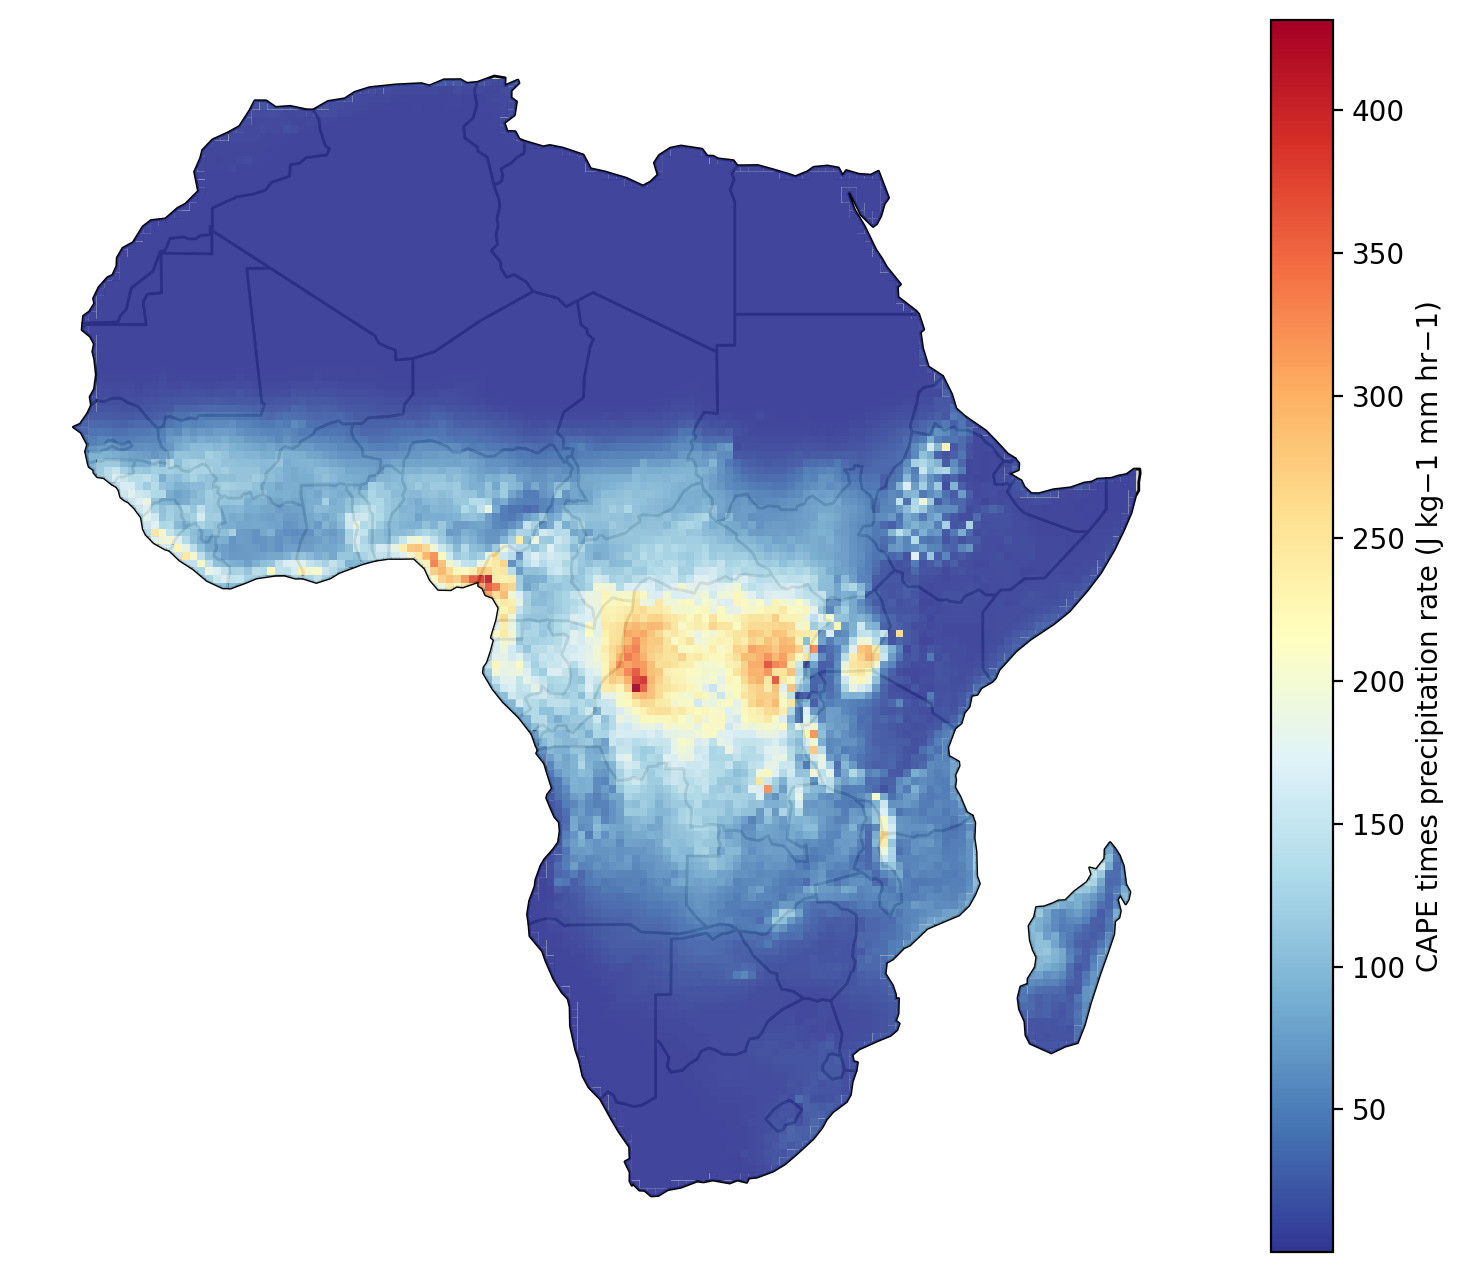
\includegraphics[width=\textwidth]{CAPEp_21.02.png}
    \captionof{figure}{Map showing 2014-18 mean lightning measure (CAPE $\times$ precipitation) values}
    \label{fig:map}
  \end{minipage}
  \end{adjustwidth}
\end{table}

\section{Methodology} \label{sec:methodology}
I use different methodologies to study the labour supply channel and the net effect of outages on employment. Section~\ref{subsec:lsmethod} discusses the methodology I use to study the labour supply channel. I employ logit with an interaction term between blackouts and an item being electric. Section~\ref{subsec:nemethod} discusses my methodology in studying the net effect of outages. I employ an IV strategy with interaction terms between outages and gender/skill. 
\subsection{Labour Supply Channel} \label{subsec:lsmethod}
In this part, I investigate whether there is evidence that electricity outages affect labour supply via household decisions to purchase electric appliances. Dinkelman (2011) \cite{dinkelman2011a} finds electrification in South Africa to be associated with higher household usage of electric lighting and cooking, but not other, non-electric, appliances like a flush toilet. Could electricity blackouts have a similar effect? To explore if the association between blackouts and the probability of an item being owned differs for electric versus non-electric items, I estimate the following logit regression. I use logit, as opposed to OLS, because my dependent variable is binary, taking value 1 if an item is owned, and 0 otherwise. 
\begin{adjustwidth}{-0.4in}{-0.4in}
\small
\begin{equation} \label{eq:eq1}
\log\left(\frac{\Pr(\text{\textit{item\_owned}}_{ih} = 1)}{1 - \Pr(\text{\textit{item\_owned}}_{ih} = 1)}\right) = \alpha_0 + \alpha_1 blackouts_{h} + \alpha_2 electric_{ih} + \alpha_3 blackouts \times electric_{ih} + \alpha_4 \textbf{X}_{h} + \gamma_{s} + \epsilon_{ih}
\end{equation}
\normalsize
\end{adjustwidth}
\par
For item \textit{i} in household \textit{h}\footnote{Running regressions at item-household level increases my sample size 34-fold relative to regressions at household level (1,250 households $\times$ 34 categories = 42,500).}. $\textbf{X}_{h}$ is a vector of household controls - urban, household head (HH) sex, HH age, last payment from main job, distance to major road, mean temperature, total precipitation\footnote{I include temperature and precipitation because weather matters for agricultural household income, which may not be reflected in a question about payments from a job for self-employed workers or those not being paid in cash.} - and $\gamma_{s}$ is a state (of Nigeria) fixed effect. The coefficient of interest is $\alpha_{3}$, which tells us whether the association between blackouts and ownership of an item depends on whether it is electric. 

\subsection{Net Effect of Outages on Employment} \label{subsec:nemethod}
In the second part of this paper, I estimate the \textit{net} effect of outages on employment by gender, which is the resultant of labour supply and demand forces. I use an instrumental variable strategy to identify the causal link\footnote{In this section, I extend Mensah's (2024) \cite{mensah2024a} strategy. I follow Mensah in 1) data sources, 2) instrumental variable, 3) most controls and fixed effects. However, extend and adapt Mensah's design. To analyse vulnerability to outages by gender and skill, I include interaction terms of gender and skill with outages and controls. Instead of a dummy variable for outages, my main regressions use a percentage measure, to avoid the arbitrary cutoff Mensah's uses for sorting into two groups. For the dependent variable, I use a 0/0.5/1 measure of employment, separating full-time and part-time employment, unlike Mensah. I also include an urban/rural dummy as a control (significant at 10\%).}. I instrument for electricity outages using a measure of lightning strikes at the community (PSU) level\footnote{I use the community level for my instrument because the Afrobarometer Survey is geocoded, but only at community level. Thus, I can only associate my lightning variable with community coordinates.}.
\par
Why do I need to use an IV? OLS estimators, even with the controls I include below, would be prone to bias due to omitted variables, simultaneity, and measurement error. Thus, the resulting estimates could not be interpreted as causal. Omitted variables could include wealth or income (which I cannot control for, as they are not part of the Afrobarometer dataset). Income is likely to be negatively associated with outages, as firms and households use self-generated electricity to limit vulnerability to outages \cite{steinbuks2010a}. However, the direction of the association between income and employment is not obvious \cite{grogan2013a}: it depends on the relative size of the income and substitution effects, as well as household preferences for labour versus leisure. Income being negatively (positively) associated with employment would bias the estimator for outages upwards (downwards). There is also a risk of simultaneity, because non-payment is more likely in high-unemployment, low-income areas, in turn leading to outages \cite{dzansi2018a}. Determining the sign of simultaneity bias is not simple and would require us to estimate the two-equation structural model for blackouts and employment \cite{wooldridge2020a}. Finally, measurement error of outages, due to the measurement error being survey responses, would cause attenuation bias, biasing estimators towards zero. 
\par	
The instrument I use is a measure of lightning strikes. Lightning is used as an instrument for outages by Mensah (2024) \cite{mensah2024a} and Andersen and Dalgaard (2013) \cite{andersen2013a}. It is a relevant instrument (as shown in Table~\ref{tab:firststagereg}) because when lightning strikes electricity transmission infrastructure, a voltage surge occurs, damaging the infrastructure and causing an outage until it is repaired. Concerning exclusion, lightning, being a natural phenomenon, is not caused by economic or institutional factors. Despite this, the exclusion condition could be violated through two channels. First, through agriculture: temperature and precipitation both contribute to lightning and affect agricultural employment, as crop performance is dependent on weather \cite{taraz2021a}. Secondly, lightning may limit the diffusion of mobile technologies \cite{manacorda2020a}, which in turn hampers economic growth and employment. I thus control for cell phone service and logs of mean annual temperature and total precipitation, arguing that given these controls, the exclusion condition is likely satisfied. My main regression equations are as follows.
\par
\noindent IV First Stage:
\begin{equation}
outages_{ijct} = \alpha_0 + \alpha_1 ln(lightning)_{jct} + \alpha_2 ln(lightning) \times female_{ijct} + \alpha_3 \textbf{X}_{ijct} + \gamma_{c} + \delta_{t} + \lambda_{i} + \epsilon_{ijct}
\end{equation}
\begin{equation}
outages \times female_{ijct} = \pi_0 + \pi_1 ln(lightning)_{jct} + \pi_2 ln(lightning) \times female_{ijt} + \pi_3 \textbf{X}_{ijct} + \gamma_{c} + \delta_{t} + \lambda_{i} + \eta_{ijct}
\end{equation}
\par
\noindent For individual \textit{i} at time \textit{t} in community \textit{j} in country \textit{c}. Where: $outages_{ijct}$ is a measure of outages; $ln(lightning)_{jct}$ is the logarithm of lightning; $\textbf{X}_{ijct}$ is a vector of controls - age, age squared, gender, urban, cell phone service, and logs of average annual temperature and total precipitation; $\gamma_c$ is a country fixed effect; $\delta_t$ is a year fixed effect; and $\lambda_{i}$ is an education fixed effect. To verify the relevance condition, we look at the sign and significance of $\alpha_1$ and $\pi_2$.
\par
\noindent IV Second Stage:
\begin{equation} \label{eq:eq4}
employment_{ijct} = \beta_0 + \beta_1 \widehat{outages}_{ijct} + \beta_2 \widehat{outages \times female}_{ijct} + \beta_3 {female}_{ijct} + \beta_4 \textbf{X'}_{ijct} + \gamma_{c} + \delta_{t} + \lambda_{i} + u_{ijct}
\end{equation}
\par
\noindent $\textbf{X'}_{ijct}$ is a vector of controls (same as above) \textit{and} interactions of age, age squared, and cell service with female. My two coefficients of interest for this specification are $\beta_1$ and $\beta_2$. The first is the estimated effect of outages on employment for males. The second is the estimated difference between the effect for females and males: the sign and significance of $\beta_2$ will indicate whether the effect of outages on employment is stronger for males or females. In the extension where I consider how skill affects vulnerability to outages, I further include \textit{skilled} as a control, as well as adding interaction terms of \textit{skilled} with \textit{outages}, \textit{female} (and age, age squared, and cell service), which I interpret similarly. I do not control for \textit{skilled} in my main specification, because it significantly reduces the sample size.

\subsubsection{First Stage}
\noindent Table~\ref{tab:firststagereg} shows first stage regression estimates for two of my instrumented variables: outages and an interaction term between outages and female\footnote{I similarly find instrument validity for my 2 other instrumented variables: \textit{outages}$\times$\textit{skilled} and \textit{outages}$\times$\textit{skilled}$\times$\textit{female}. Available upon request.}. It shows a significant (at 1\%, in both cases) association with the instrument: \textit{Ln(lightning)}, the log of my lightning measure, in the first case, and \textit{Ln(lightning)}$\times$\textit{female} in the latter case. For example, in column 1, I find that a 1\% increase in lightning intensity is associated with a 0.102 percentage point increase in the share of households experiencing outages. The F statistic is above 10, i.e., the typical cutoff for concern about weak instrument bias,  in both cases.
\begin{table}[htbp]
  \begin{adjustwidth}{-0.4in}{-0.4in}
  \centering
  \footnotesize
  \begin{minipage}[t]{0.60\textwidth}
    \vspace{5pt}
    \centering
    % Table with left-aligned first column
    \caption{First stage regressions}
    \label{tab:firststagereg}
    \begin{tabular}{l c c}
        \hline\hline
        \centering
        & Outages (\%) & Outages (\%) $\times$ Female \\
        \cline{2-3}
        & (1) & (2) \\
        \hline
        Ln(lightning) & 10.19*** & 0.381\\
        & (1.604)& (0.923)\\
        Ln(lightning) $\times$ Female & -0.121& 8.611***\\
        & (0.122)& (0.889)\\
        \hline
        F statistic & 21.50&  59.88\\
        Observations     &   32,277   &  32,277   \\
        \hline
        \end{tabular}
        \begin{flushleft}
        \scriptsize
        * Significant at 10\% ** Significant at 5\% *** Significant at 1\%. Controls: age, age squared, gender, urban, cell phone service, and logs of average annual temperature and total precipitation. Fixed effects: country, year, and education. Standard errors clustered at city level.
        \end{flushleft}
  \end{minipage}
  \hfill
  \begin{minipage}[t]{0.49\textwidth}
    \vspace{0pt}
    \centering
    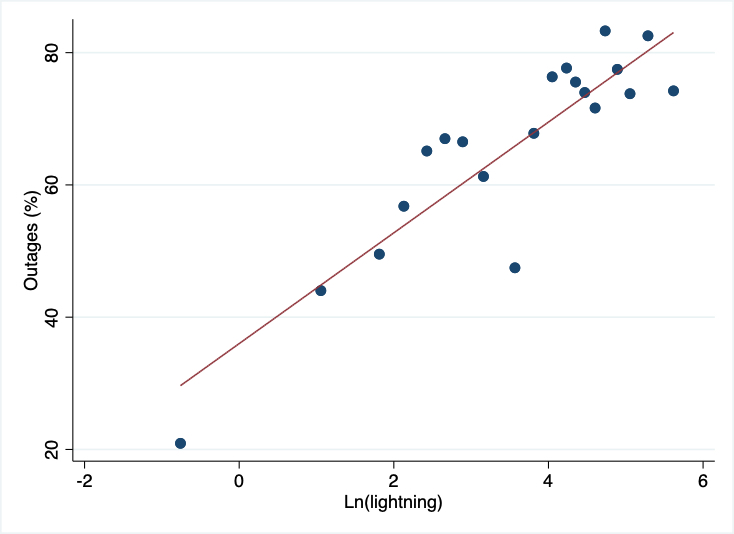
\includegraphics[width=\textwidth]{firststage final.jpg}
    \captionof{figure}{Binned scatterplot showing positive association between lightning and outages}
  \end{minipage}
    \end{adjustwidth}
\end{table}

\section{Results} \label{sec:results}
I am interested in estimating the effect of outages on employment and identifying particularly vulnerable groups. I first explore a hypothesis that outages affect market labour supply, especially by women, by changing purchase decisions concerning electric household appliances. Section~\ref{subsec:lsresults} discusses my logit estimates: in support of the household labour supply channel, I find that blackouts are negatively associated with the probability of owning electric items, but not non-electric items. I then estimate the net causal effect of outages on employment, by gender and skill. In Section~\ref{subsec:neresults}, I find that males - especially skilled - are most affected by outages. I argue that this surprising exposure of men to outages, despite a likely \textit{stronger} supply-side effect for women, can in part be explained by occupational differences between women and men, which cause biased demand-side effects. Women are more often employed in services than men, and less often in manufacturing, thus lowering their vulnerability to outages, which impact energy-intensive production \cite{alam2013a}.
\subsection{Labour Supply Channel} \label{subsec:lsresults}
In this section, I verify the hypothesis that electricity blackouts are associated with decisions about electric appliance purchases, which in turn likely influence household time allocation between home production and market labour. To this end, in column 2 of Table~\ref{tab:results1} below I estimate equation~\ref{eq:eq1} (column 1 is a naive version excluding an interaction term, for comparison). The results suggest that given controls, the association between blackouts and the probability of a household owning an item is indeed significantly more negative for electric items. While my estimates cannot be interpreted as causal, they do provide support for the the hypothesized labour supply channel, which requires a negative association between blackouts and ownership of electric items. With the appliance-household labour supply channel, we
would expect blackouts to decrease market labour supply and for this effect to be stronger for women.
\par
To analyze whether blackouts are associated with decisions about electric appliance purchases, I am interested in the interaction term between \textit{blackouts} and \textit{electric}. It indicates that association between blackouts and probability of ownership is significantly more negative for electric items relative to non-electric items. However, log-odds estimates cannot be interpreted as marginal effects. Instead, I calculate average marginal effects (AME). The AME of blackouts is approx. 0.6 percentage points (pp) for non-electric items (varies depending on the combination of dummy variables), and approx. -0.3 pp for electric items. This means that an increase in the frequency of blackouts by one (category), e.g. from yearly to monthly, or monthly to weekly, is associated with an approx. 0.3 pp lower probability of ownership for an electric item. The margin plots in Figure~\ref{fig:marginplots1}, which show how the probability that an item is owned changes with blackouts for average households with different combinations of urban and female dummies, show the same pattern. Blackouts are associated with increasing probability of owning a non-electric item, and decreasing probability of owning an electric item.
\par
These results are aligned with the hypothesis that households may respond to blackouts by purchasing fewer electric appliances. If blackouts directly matter for the decision to purchase electric items, such as a TV or a washing machine, we would expect a negative association between blackouts and ownership for electric items - as I indeed find. Moreover, the insignificant relationship for non-electric items (given controls) suggests it is unlikely that the estimates for \textit{blackouts} are reflecting the effect of an omitted variable. What does this mean for the expected effect of outages on employment? Reduced purchases of electric appliances (in response to blackouts) are likely to cause lower market labour supply, especially for women (who tend to be responsible for home production), as home production takes longer and households' “effective days” shrink, leaving less time for market labour (assuming income effect dominates). We would thus expect blackouts to decrease market labour supply and this effect to be stronger for women. Taken in isolation, i.e., ignoring possible gender bias on the demand side, this would lead us to expect that the net negative effect of outages on employment would be stronger for women than men. 
\par \noindent
\textit{\textbf{Key takeaways:} I find that the association between electricity blackouts and the probability of owning an item is significantly more negative for electric items. This is in line with the hypothesis that blackouts may influence decisions about electricity appliance purchases (e.g., fridge, microwave, washing machine). In turn, lower appliance ownership is likely to decrease market labour supply, especially of women, as households become less productive at home production and hence have less time remaining for market labour. Focusing on the labour supply side in isolation, we would thus expect women's employment to be more vulnerable to outages than men's.}
\par
\begin{table}[htbp]
  \centering
  \footnotesize
    \vspace{5pt}
    \centering
    % Table with left-aligned first column
    \caption{Logit regression estimates}
    \label{tab:results1}
    \begin{tabular}{lcc}
        \hline\hline
        & \multicolumn{2}{c}{Item Owned (0/1)} \\
        \cline{2-3}
        Log-odds coefficients& (1) & (2) \\
        \hline
        Blackouts  & 0.00543  & 0.0275 \\
        & (0.016)   & (0.018) \\
        Electric Item & -0.362*** &   -0.225*** \\
        & (0.029) & (0.077) \\
        Blackouts $\times$ Electric &   & -0.0414**  \\
        &  & (0.021) \\
        \hline
        Log pseudolikelihood & -26,807  & -26,805 \\
        Observations     &    42,500    &  42,500   \\
        \hline
    \end{tabular}  
    \begin{flushleft}
    \scriptsize
    * Significant at 10\% ** Significant at 5\% *** Significant at 1\%. Controls: urban, female HH, income, age HH, KMs to major road, temperature, precipitation. Standard errors clustered at local government area level.
    \end{flushleft}
\end{table}
\begin{centering}
    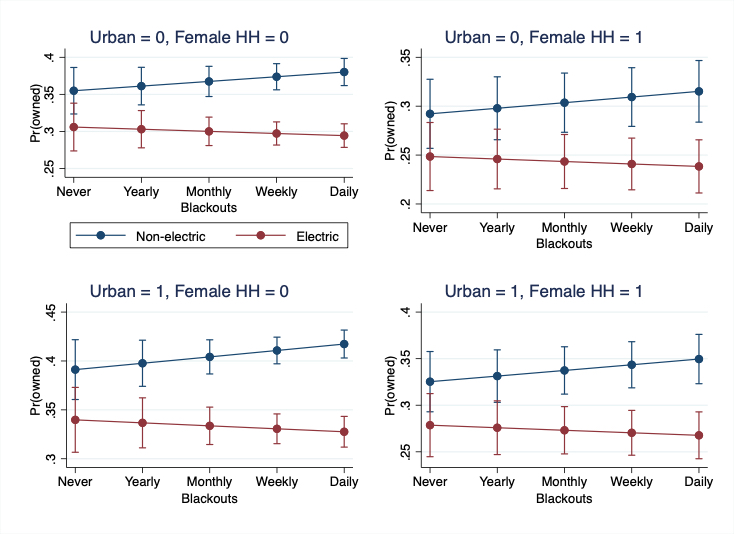
\includegraphics[width=0.7\textwidth]{GHS graphs final.jpg}
    \captionof{figure}{Margin plots showing change in probability of owning an item with blackouts} 
    \label{fig:marginplots1}
\end{centering}

\newpage
\subsection{Net Effect of Outages on Employment} \label{subsec:neresults}
Having explored the labour supply side, I now estimate the net causal effect of outages on employment for different gender and skill groups. In Section~\ref{sec:genderskill}, I identify skilled males as most vulnerable. In Section~\ref{sec:demand}, I argue that occupational differences are partly responsible for this effect.

\subsubsection{Results by Gender and Skill} \label{sec:genderskill}
In Table~\ref{tab:mainresults}, we immediately observe that for both OLS and IV specifications\footnote{Note: In Table~\ref{tab:mainresults}, my OLS estimates in columns 1 and 2 are closer to zero/more positive than the IV estimates in columns 3 and 4. This may be due to OLS being biased towards zero due to omitted variable bias or attenuation bias, or because because my IV estimates reflect Local Average Treatment Effect (LATE), which is larger than Average Treatment Effect (ATE). IV identifies the effect for the subgroup of the population where the treatment (outages) is associated with the instrument (lightning), which may have unique characteristics (e.g., weak grid infrastructure) that make it more affected, leading to large estimated effects compared to the general population. In the analysis above, I am discussing LATE.}, the effect of outages is significant and negative for male employment, and it is significantly \textit{less} negative for females. The main column of interest is 4, in which I estimate equation~\ref{eq:eq4}. It suggests that a 1 pp increase in the share of households in a community facing outages reduces the probability of employment by a significant (at 5\%) 0.217 pp for males and an insignificant 0.102 pp for females, as the effect is 0.115 pp closer to 0 (i.e., less negative) for females (significant at 1\%). Men being more vulnerable is a surprising, though not impossible, result. It is surprising given the literature on the effects of \textit{electrification}, which tends to find larger effects for women \cite{dasso2015a} \cite{dinkelman2011a} \cite{grogan2013a}, and my results in Section~\ref{subsec:lsresults}, which provided support for a household labour supply channel, which is likely to be stronger for women, who perform more labour at home. The net effect I identify here is the opposite. To explore this interesting result, I want to understand how skill fits into this.
\par
Table~\ref{tab:skill} provides an answer. In column 4, we see that while the effect of outages more negative for skilled workers\footnote{This is in line with Mensah (2024), who, using subsample analysis, only finds a significant effect for skilled workers.}, being female mitigates this effect. As a male, being skilled is associated with a predicted 0.136 pp larger decline in probability of employment in response to outages than if one were unskilled, whereas for females, this difference is only 0.095 pp. This allows us to break down the “protective” effect of being female, identified in Table~\ref{tab:mainresults}, into two channels: it both directly interacts with outages \textit{and} decreases the vulnerability associated with being skilled. Overall, the effect of outages on employment is strongest for skilled males, then unskilled males, then skilled females, and, finally, it is weakest for unskilled females. 
\par \noindent
\textit{\textbf{Key takeaways}: Estimating the net effect of outages on employment, I find that being male and being skilled are sources of vulnerability. This is surprising given that on the labour supply side, we expect women to be more impacted. The contrast between the total effect and the supply channel suggests that demand-side effects are likely to be driving the net result.}

\newpage
\begin{table}[htbp]
\centering
\footnotesize
\caption{Results by Gender}
\label{tab:mainresults}
\begin{tabular}{lcccc}
\hline\hline
& \multicolumn{4}{c}{Employment (0/0.5/1)} \\
\midrule
& \multicolumn{2}{c}{OLS} & \multicolumn{2}{c}{IV} \\
& (1) & (2) & (3) & (4) \\
\midrule
Outages (\%) 
  & -0.000500*** 
  & -0.000736*** 
  & -0.00167* 
  & -0.00217** \\
& (0.0001) & (0.0001) & (0.0009) & (0.0009) \\[6pt]
Female (0/1)
  & -0.0684***  
  & -0.0426 
  & -0.0688***  
  & -0.0909 \\
& (0.006) & (0.050) & (0.006) & (0.058) \\[6pt]
Outages $\times$ Female
  &  
  & 0.000508***
  &  
  &  0.00115*** \\
&  & (0.0002) &  & (0.0004) \\[6pt]
\midrule
Mean dependent variable
  & 0.580 
  &  0.580  
  & 0.580 
  & 0.580 \\
Adjusted R\textsuperscript{2}
  & 0.188 
  &  0.188  
  & --- 
  & --- \\
Kleibergen--Paap rk Wald F stat
  & --- 
  & ---
  & 39.585 
  & 19.682 \\
Pr $>$ F & 0.0000 & 0.0000 & 0.0000 & 0.0000 \\
Observations 
  & 32,277  
  & 32,277  
  & 32,277
  & 32,277\\
\midrule
\bottomrule
\end{tabular}
\end{table}
\begin{flushleft}
\footnotesize
* Significant at 10\% ** Significant at 5\% *** Significant at 1\%. Same controls and fixed effects as in Table~\ref{tab:firststagereg}. In (2) and (4), I interact female with age, age squared, and cell service. Standard errors clustered at city level. 
\end{flushleft}

\begin{table}[!htbp]
\centering
\footnotesize
\caption{Results by Gender and Skill}
\label{tab:by skill}
\label{tab:skill}
\begin{tabular}{lcccc}
\hline\hline
& \multicolumn{4}{c}{Employment (0/0.5/1)} \\
\cmidrule(lr){2-5}
& \multicolumn{4}{c}{IV} \\
 & (1) & (2) & (3) & (4)\\
\midrule
Outages (\%)
  & -0.00113
  & -0.000740
  &  -0.00109
  & -0.000993 \\
  & (0.0009)
  & (0.0001)
  & (0.0009)
  & (0.0009)\\[3pt]
Female (0/1)
  & -0.0323***
  & -0.0327***
  &  -0.126*
  & -0.114\\
  & (0.006)
  & (0.006)
  & (0.076)
  & (0.075)\\[3pt]
Skilled (0/1)
  & 0.160***
  & -0.239***
  & -0.254***
  & -0.252***\\
  & (0.009)
  & (0.088)
  & (0.088)
  & (0.088)\\[3pt]
Outages $\times$ skilled
  & 
  & -0.00123**
  & -0.00113** 
  & -0.00136** \\
  & 
  & (0.0006)
  & (0.0006)
  & (0.0006)\\[3pt]
Outages $\times$ female
  & 
  & 
  & 0.00062
  & 0.00046 \\
  & 
  & 
  & (0.0005)
  & (0.0005)\\[3pt]
Outages $\times$ skilled $\times$ female
  & 
  & 
  & 
  & 0.000414** \\
  & 
  & 
  & 
  & (0.0002)\\[3pt]
\midrule
Mean dependent variable
  & 0.641 
  &  0.641  
  & 0.641 
  & 0.641 \\
Kleibergen--Paap rk Wald F stat
  & 33.781 & 16.911  & 11.313 
  & 8.505 \\
Pr $>$ F & 0.0000 & 0.0000 & 0.0000 & 0.0000 \\
Observations 
  & 19,628  & 19,628 & 19,628 & 19,628\\
\midrule
\bottomrule
\end{tabular}
\end{table}
\begin{flushleft}
\footnotesize
* Significant at 10\% ** Significant at 5\% *** Significant at 1\%. Same controls and fixed effects as in Table~\ref{tab:firststagereg}. In columns (2), (3) and (4), I interact skilled, female, and both, respectively, with  age, age squared, and cell service. Standard errors clustered at city level.
\end{flushleft}
\par
\subsubsection{Labour Demand and Occupational Differences by Gender} \label{sec:demand}
\noindent In this section, I argue that a demand-side channel is responsible for part of the gender disparity in vulnerability to outages. On the labour demand side, outages increase firm costs and lower productivity, decreasing demand for labour. Which firms are most affected by outages? Those in energy-intensive industries \cite{alam2013a}. In a developing context, this especially includes firms engaged in manufacturing with machinery (e.g., rice and steel mills \cite{alam2013a}). Females may be less vulnerable to outages partly because, regardless of skill level, they are more likely to be employed in services than males, and less likely to be employed in manufacturing\footnote{This is illustrated in Table~\ref{tab:occupationstats}, but also supported by other research. Baccini et al. (2021) \cite{baccini2021a} find that in Africa, women make up 40\% of workers in services, twice as much as in manufacturing.}. Sectoral composition also helps explain why being female limits the vulnerability to outages that comes with being skilled: for men, becoming skilled is most often associated with obtaining energy-intensive manufacturing jobs, whereas women are just as likely to go into mid-level professional jobs in services.
\par
The Afrobarometer dataset is not granular enough to permit direct identification of workers in energy-intensive industries. However, the occupational breakdown by gender, presented in Table~\ref{tab:occupationstats}, provides some insight. The Artisan or skilled manual worker (e.g., mechanic, \textit{machinist} or skilled manufacturing worker) category most likely includes workers in energy-intensive manufacturing. It makes up almost 18\% of male, but only 11\% of female employment. It is also the largest category for skilled males by a large margin, whereas Mid-level professional (e.g., teacher, nurse, mid-level government officer) is most popular among skilled females\footnote{Albeit by a thin margin over Artisan or skilled manual worker.}. This helps explain why females are less vulnerable to outages than males, and why \textit{skilled} females are less vulnerable than skilled males\footnote{The breakdown also shows why skilled workers in general are more exposed. Manual workers operating machines (machinists) fall into the skilled category, whereas the unskilled includes cleaners, laborers, and domestic help (unskilled manual), housewives/homemakers, agricultural workers, and vendors (examples from Afrobarometer) - all non-energy-intensive.}. 
\par
Occupational differences could thus be responsible for a gender-biased demand-side channel, whereby men, on average, are more exposed to outages. This helps us understand why the net effect of outages (men more impacted) differs from what supply-side arguments would lead us to expect (women more impacted). Thus, I argue that vulnerability differences by gender stem in part from occupational differences. However, Table~\ref{tab:occupcontrol} suggests that this is part of, but not \textit{the whole} story. Column 1 estimates equation~\ref{eq:eq4}, but for a smaller sample than in Table~\ref{tab:mainresults} (excluding those with missing occupation). The gender difference is present, though not significant (possibly due to smaller sample). In column 2, I include an occupation fixed effect, and find that the magnitude of the gender difference decreases, from 0.0891 pp to 0.0731 pp. Hence, occupation seems to account for only part of the gender disparity in this simple setup.
\par \noindent 
\textit{\textbf{Key takeaways:} On the demand side, we expect employment of workers in energy-intensive industries to be most vulnerable to outages. An occupational breakdown suggests that males are more likely to work in such industries than women. Therefore, occupational differences are likely part of the gender vulnerability story. However, while controlling for occupation lowers the magnitude of the gender difference, it does not completely eliminate it.}

\begin{table}[htbp]
  \begin{adjustwidth}{-0.4in}{-0.4in}
  \centering
  \scriptsize
  \begin{minipage}[t]{0.65\textwidth}
    \caption{Occupational breakdown by gender}
    \label{tab:occupationstats}
    \begin{tabular}{l c c c c}
        \hline\hline 
        &    \multicolumn{2}{c}{Male} &    \multicolumn{2}{c}{Female} \\
    \cmidrule(lr){2-5}
    &   Number & Share (\%) &    Number & Share (\%)  \\
    \hline
    \multicolumn{5}{c}{Skilled}\\
    \hline
    Housewife/homemaker &292 &3.13 & 890& 8.64\\
    Agriculture/farming/fishing/forestry &1,878 & 20.14& 1,741& 16.90  \\
    Trader/hawker/vendor &980 & 10.51  & 1,792&  17.39 \\
    Retail/shop & 452&4.85 & 668&6.48 \\
    Unskilled manual worker & 1,572&16.86  & 1,489 & 14.45\\
    \hline
    \multicolumn{5}{c}{Unskilled}\\
    \hline
    Artisan or skilled manual worker &1,672 & 17.93&1,133 & 11.00 \\
    Clerical or secretarial & 236 & 2.53&  447& 4.34\\
    Supervisor/foreman/senior manager & 321 & 3.44&232  &2.25 \\
    Security services  & 459&4.92 & 313& 3.04 \\
    Mid-level professional & 969& 10.39& 1,141& 11.08\\
    Upper-level professional & 495&  5.31& 456& 4.43\\
    \hline
    Total   &    9,326 &           100\% & 10,302&           100\%\\
    Of which unskilled & 5,175 & 55.49 & 6,579 & 63.86 \\
    Of which skilled &4,151& 44.51 & 3,723& 36.14 \\
    \midrule
    \bottomrule
    \end{tabular}
    \end{minipage}
  \hfill
  \begin{minipage}[t]{0.45\textwidth}
      \caption{Controlling for occupation}
    \label{tab:occupcontrol}
    \begin{tabular}{lcc}
        \hline\hline
        & \multicolumn{2}{c}{Employment (0/0.5/1)} \\
        \cline{2-3}
        & \multicolumn{2}{c}{IV} \\
        & (1) & (2) \\
        \hline
        Outages (\%) 
  & -0.00155* 
  &  -0.00156*\\
& (0.0009) & (0.0009) \\[6pt]
Female (0/1)
  & -0.0885 
  &  -0.0829\\
& ((0.078) & (0.079) \\[6pt]
Outages $\times$ Female
  &  0.000891
  &   0.000731\\
 & (0.0005) & (0.0005) \\[6pt]
\midrule
Occupation Fixed Effect
  &  No
  &  Yes \\
\midrule
Mean dep. var.
  &  0.547
  &  0.547 \\
Pr $>$ F & 0.0000 & 0.0000 \\
Observations  
  & 19,628
  & 19,628\\
        \hline
    \end{tabular}  
        \begin{flushleft}
        \scriptsize
        * Significant at 10\% ** Significant at 5\% *** Significant at 1\%. Same controls and interactions as in Table~\ref{tab:mainresults}. Standard errors clustered at city level.
        \end{flushleft}
    \end{minipage}
      \end{adjustwidth}
\end{table}

\section{Conclusion} \label{sec:conclusion}
The aim of this study has been to identify costs associated with electricity outages to motivate and inform investments in electricity reliability. In particular, I estimate the impact of outages on equilibrium employment and seek to identify particularly vulnerable groups, by gender and skill.
\par
I first explored a labour supply channel linking outages with employment through the former's effect on electric appliance purchases. This was a natural starting point in comparing effects for men and women, because home production is gender-biased: women tend to be responsible for more of it. My analysis provided some support for this channel, as I found that the association between blackouts and the probability of owning an item is significantly more negative for electric items. This led me to expect a stronger negative effect of outages for women's equilibrium employment (if we naively assumed that demand-side effects would not be gender-biased), as they are more likely to sacrifice market employment in response to an increased home production burden. 
\par
However, when I estimated the net, causal, effect of outages for employment, I found the opposite: the negative effect of outages is significantly stronger for males. To reconcile these results, I incorporated labour demand considerations. I argued that gender differences in sectoral composition are responsible for part of the effect we see. Electricity-intensive sectors, such as manufacturing, are more impacted by outages \cite{alam2013a}, and women, regardless of skill level, are less likely to work in manufacturing, and more likely to work in services, than men \cite{baccini2021a}. Vulnerability to electricity outages is therefore both a story of gender and of occupation. Regarding policy implications, this paper suggests that in developing countries, skilled male workers have the most to gain from projects oriented at improving electricity reliability.

\newpage
\section{Appendix}
\subsection*{Robustness}
\textbf{Labour Supply Channel}
\par
\begin{itemize}
\item An important result for robustness is that \textit{blackouts} are not significantly associated with the probability of owning a non-electric item. This gives confidence the estimated coefficient for \textit{blackouts} is not reflecting some omitted variable's effect. 
\item  I use robust, cluster-adjusted (at local government level) standard errors, thus not needing to test for heteroskedasticity. With this sample size, by the Central Limit Theorem, errors are asymptotically normally distributed. 
   \item I verify if estimates are aligned with previous research and economic theory. Firstly, as expected given that electric items are often more expensive than non-electric alternatives \cite{koehlin2011a}, irrespective of blackouts, an item being electric has significantly lower probability of ownership. Moreover, I find that households with higher income are more likely to own an item. So are urban households, which might reflect better credit access, repair services, and resale markets \cite{jalan2002a}. These sense checks provide indication of the accuracy of my data cleaning and analysis (results table including estimates for controls available upon request).
    \item I find a Variance Inflation Factor (VIF) of an OLS regression excluding my interaction terms (which cause multicollinearity) of 3.35, which is below the rule-of-thumb threshold of 10. Multicollinearity is unlikely.
    \item There remains some risk of endogeneity, primarily due to omitted variables. These could include appliance availability/price, household preferences, or access to credit, which are not in the GHS dataset. Given several unobservables, it is difficult to conclude the direction of bias. Using an IV for outages would be an improvement.
\end{itemize}
\textbf{Net Effect of Outages on Employment}
\begin{itemize}
\item I used robust, cluster-adjusted standard errors at city level, high-dimensional year, country, and education fixed effects, controls, and winsorized variables. 
\item  I also experimented with 1) one versus multiple interaction terms with gender and 2) subsample analysis, not finding any significant results that would conflict with my main results.
    \item I conducted a subgroup placebo test using communities with a 0\% electrification rate (sample size is 7,361). For these households, we would expect lightning to not be associated with employment given controls (same as in Table~\ref{tab:firststagereg}), since the outage channel is not present. Indeed, the coefficient on \textit{Ln(lightning)} is positive and not significantly different from 0 (table available upon request).
        \item I tested for functional form misspecification using Ramsey RESET. The squared and cubed predicted values are jointly insignificant, with Prob $>$ F = 0.2029, so I do not reject the null hypothesis that the model is well-specified.
    \item The mean VIF for an OLS regression without interaction terms is 6.46, which is below the rule-of-thumb threshold of 10. Multicollinearity is unlikely.
\end{itemize}

\newpage
\renewcommand\refname{Data Sources}
\begin{thebibliography}{9}

\bibitem{ghs}
National Bureau of Statistics (NBS). General Household Survey, Panel  2012-2013, Wave 2. World Bank, Development Data Group. \href{https://doi.org/10.48529/KXPY-AA72}{https://doi.org/10.48529/KXPY-AA72}.
\bibitem{afrobarometer}
Afrobarometer Data, Merged Data, Rounds 6 and 7, 2014–15 and 2016–18. Available at \url{http://www.afrobarometer.org}\footnote{Geocoded dataset is only available upon request, so I have submitted my raw data.}.
\bibitem{cds}
Hersbach, H., Bell, B., Berrisford, P., Biavati, G., Horányi, A., Muñoz Sabater, J., Nicolas, J., Peubey, C., Radu, R., Rozum, I., Schepers, D., Simmons, A., Soci, C., Dee, D., Thépaut, J-N. (2023): ERA5 monthly averaged data on single levels from 1940 to present. Copernicus Climate Change Service (C3S) Climate Data Store (CDS), DOI: \href{https://doi.org/10.24381/cds.f17050d7}{10.24381/cds.f17050d7}.
\end{thebibliography}
\nocite{*}
\renewcommand\refname{References}
\bibliography{anystyle-2-2}

\end{document}
